\subsection{DMA Engine}
\begin{figure}[t]
\begin{center}
\includegraphics[scale=1.4]{../../img/dma-tx.pdf}
\caption{DMA engine: Transmission channel}
\label{fig:dma-tx}

\end{center}
\end{figure}


Both the baseline and accelerated systems feature a direct memory access
(DMA) engine for transferring Ethernet frames to and from main memory.
A significant increase in I/O performance is realized by minimizing the
involvement of the processor, exploiting a wider memory interface for
improved throughput, and avoiding pollution of the inner caches.
The DMA engine attaches directly to the media access controller of the
NIC in the baseline, and alternatively to the traffic manager with the
accelerator present.

The DMA engine comprises two simplex channels dedicated to receive (Rx)
and transmit (Tx).
A channel is internally structured as a pair of ingress and egress
units, respectively designated the \emph{front-end} and \emph{back-end},
which coordinate by ready/valid handshaking to exchange blocks of data.
Each end fully encapsulates the protocol-specific logic for its
external interface and presents a generic FIFO abstraction at the other
terminal, enabling units of different types to connect and interact in a
consistent modular fashion.
The design is thus intended to accommodate a variety of peripheral
interfaces through interchangeable sets of front-ends and back-ends.

The memory units do not directly interface with the DRAM controller but
instead communicate with the L2 coherence agent through the TileLink
protocol, the primary on-chip system interconnect.
This layer normally mediates access to the shared last-level cache, if
present, or to main memory otherwise, as in this case.
Closer integration with the cache hierarchy, although perhaps
unconventional for peripheral I/O, simplifies cache coherence in a
system-on-chip environment:
The DMA engine is treated as simply another client like a processor
tile.
By marking DMA requests as uncached, the coherence agent ensures that
all necessary cache flushes and invalidations occur on behalf of the DMA
engine, which conveniently avoids interaction with coherence traffic.

Each TileLink transaction delivers a 64-byte cache line and supports
access to the complete 32-bit physical address space, thus eliminating
the need for bounce buffers.
The exact widths of TileLink addresses and data are configurable
system-level parameters.

One possibility briefly considered but left unpursued is adding an
arbiter port to the L1 data cache for DMA operations.
Since a TLB already resides in the L1 cache, this would naturally
facilitate zero-copy transfers into user-mode virtual address spaces
without requiring page fixing or pinning of physical memory.
The eight-fold reduction in throughput would be somewhat compensated by
a significant improvement in latency, possibly an acceptable trade-off
given the narrow I/O width at the peripheral end.
The overriding concern, however, is cache pollution by relatively large
Ethernet frames.

\subsubsection{Transmit}

Figure \ref{fig:dma-tx} illustrates the Tx channel architecture.
The descriptor ring lists pending buffers to transmit.
To initiate a transfer, the processor enqueues a buffer descriptor with
the base address and count, which the controller then inserts into ring
at the slot denoted by an automatically incremented write pointer.
A read pointer indicates which buffer is being consumed by the channel.

Once the transfer completes, the controller raises an interrupt request.
Independent of the DMA engine, the software maintains a pointer to the
earliest descriptor yet to be acknowledged, initialized with the read
pointer after reset.
The interval from this pointer to the current read pointer,
non-inclusive, identifies the set of buffers that may be safely
deallocated.

A shallow two-entry queue decouples the front-end from the back-end.
This enables the front-end to prefetch the next cache line
simultaneously as the back-end streams the previous line.
The front-end currently serializes TileLink transactions;
although multiple outstanding requests could be pipelined as addresses
can be generated immediately, managing the potential out-of-order
arrival of responses costs extra buffer space and control logic.
In practice, this optimization proves to be largely unneeded.
After the penalty of initial load, the throughput provided by TileLink
adequately saturates the back-end to completely hide the memory latency
of 30 to 50 cycles.

\subsubsection{Receive}

\begin{figure}[t]
\begin{center}
\label{fig:dma-rx}
\includegraphics[scale=1.4]{../../img/dma-tx.pdf}
\caption{DMA engine: Reception channel}
\end{center}
\end{figure}

The Rx channel, depicted in Figure \ref{fig:dma-rx}, possesses an
architecture broadly similar to its Tx counterpart.
The descriptor ring holds the base addresses of empty buffers which have
been allocated beforehand and await to be filled with incoming frames.
A write pointer reports the next available slot and automatically
advances as descriptors are enqueued by the processor.
For simplicity, the buffers are assumed to extend to the maximum length
of an IEEE 802.3 Ethernet frame without the 802.1Q tag (1514 octets).

An internal current pointer tracks which buffer is presently active.
Upon completion of a frame, the final count is stored in a separate ring
at the slot indexed by the current pointer, while the controller raises
an interrupt request.
Counts are dequeued according to a read pointer, whose value can be used
to associate each count with the original buffer.
Note that the read pointer cannot overtake the current pointer, which
itself cannot overtake the write pointer.
Since channel activity stalls when the descriptor ring becomes empty,
the processor must resupply buffers at a rate equal to consumption.

Due to the shorter latency of store operations, the Rx front-end and
back-end do not need to be decoupled to the same degree as with the Tx
channel.
The back-end can perform the two-way TileLink acknowledgement (grant and
finish) while the front-end populates the subsequent cache line.

The existing TileLink interface omits byte-granular write masks, thus
complicating the handling of partial writes.
Consequently, receive buffers must be aligned at a cache line boundary
and, to prevent clobbering, cannot share cache lines with other data.
As the kernel network stack also expects four-byte alignment of the IPv4
header, frames are written with a two-byte initial padding.
These restrictions could be averted by resorting to read-modify-write
operations for the first and last cache lines, but this would adversely
impact latency and expose the DMA engine to coherence probes for only
minor benefits in programming convenience.
